\chapter{*Feltételes szélsőérték}

\section{Követelmények}
\begin{enumerate}
    \item Feltételes szélsőérték
    \item Szükséges feltétel (bizonyítással)
    \item Elégséges feltétel
\end{enumerate}

\section{Lokális szélsőérték és feltételei}\label{sec:loc-extr-reminder}

Ez a szekció (\ref{sec:loc-extr-reminder}) kizárólag ismétlésként szerepel, nem képezi a tárgyi tananyag részét.

\subsection{Definíció}

Legyen $1 \le n \in \N$ és $f \in \R^n \to \R$.

Ekkor $f$-nek az $a \in \dom_f$ helyen \textbf{lokális maximuma (minimuma)} van, azaz az $a$ pont egy \textbf{lokális maximumhely (minimumhely)}, ha:

$\exists K(a) = K_r(a) = \{x \in \R^n : \norm{x-a}_2 < r\}\quad (r > 0)$ amire $f(x) \le f(a) \quad (x \in K(a) \cap \dom_f)$.

Lokális minimum esetén pedig $f(x) \ge f(a)$.

Ekkor $f(a)$ az $f$ \textbf{lokális maximuma (minimuma)}.

Általánosan pedig $f$-nek az $a$-ban \textbf{lokális szélsőértéke} van, azaz az $a$ pont egy \textbf{lokális szélsőértékhelye} $f$-nek, ha $f$-nek $a$-ban lokális maximuma vagy lokális minimuma van.

\subsection{Kvadratikus alak}

Legyen $n \in \N$ és $A \in \R^{n\times n}$ szimmetrikus.

Ekkor az $A$ mátrix által meghatározott \textbf{kvadratikus alak}:

$Q \in \R^n \to \R,\ Q(x) = \dprod{Ax,\,x}\quad (x \in \R^n)$.

\subsubsection{Egy pontban kétszer differenciálható függvények}

Egy $f \in D^2\{a\}$ függvényhez az $a$-beli Hesse-mátrixból kapott kvadratikus alakot $Q_a^f$-el jelöljük, azaz:

$\displaystyle Q_a^f(x) := \dprod{f''(a)x,\,x} = \sum_{i=1}^n\sum_{j=1}^n\partial_{ij}f(a)x_ix_j \quad (x \in \R^n)$

\subsubsection{Definitség}

Egy $Q$ kvadratikus alak

\begin{enumerate}[label=(\alph*),itemsep=2pt,topsep=2pt]
    \item pozitív definit, ha $Q(x) > 0 \quad (0 \ne x \in \R^n)$
    \item negatív definit, ha $Q(x) < 0 \quad (0 \ne x \in \R^n)$
    \item pozitív szemidefinit, ha $Q(x) \ge 0 \quad (x \in \R^n)$
    \item negatív szemidefinit, ha $Q(x) \le 0 \quad (x \in \R^n)$
    \item indefinit, ha $\exists x,y \in \R^n : Q(x) < 0 < Q(y)$
\end{enumerate}

\subsection{Feltételek}

\subsubsection{Elsőrendű szükséges feltétel}

Legyen $f \in \R^n \to \R$ és tfh. egy $a \in \intp \dom_f$ helyen lokális szélsőértéke van, továbbá $f \in D\{a\}$.

Ekkor $f'(a) = \grad f(a) = \big(\partial_1f(a),\, \ldots,\, \partial_nf(a)\big) = 0$, vagyis $\partial_1f(a) = \ldots = \partial_nf(a) = 0$.

\subsubsection{Másodrendű elégséges feltétel}

Legyen $f \in \R^n \to \R$ és tfh. egy $a \in \intp \dom_f$ helyen teljesül, hogy:

\begin{enumerate}[label=(\alph*),itemsep=1pt, topsep=1pt]
    \item $f \in D^2\{a\}$
    \item $\grad f(a) = 0$
    \item $Q_a^f$ pozitív (negatív) definit
\end{enumerate}

Ekkor $f$-nek $a$-ban lokális minimuma (maximuma) van.

\subsubsection{Másodrendű szükséges feltétel}

Legyen $f \in \R^n \to \R$ és tfh. egy $a \in \intp \dom_f$ pontban:

\begin{enumerate}[label=(\alph*),itemsep=1pt,topsep=1pt]
    \item $f \in D^2\{a\}$
    \item $f$-nek az $a$-ban lokális minimuma (maximuma) van
\end{enumerate}

Ekkor $\grad f(a) = 0$ és $Q_a^f$ kvadratikus alak pozitív (negatív) szemidefinit.

\newpage

\section{Feltételes szélsőérték}

\subsection{Felvezető feladat}\label{sec:impl-example}

A következő feladat a feltételes szélsőérték és implicitfüggvények felvezetésére szolgál.

Egységnyi kerületű, $x,\ y$ oldalhosszúságú téglalapok közül keressük a legnagyobb területűt. Azaz keressük az $xy$ szorzat maximumát, ha $x>0,\ y>0$ és $2x+2y = 1$.

Legyen $f(x,y) := xy,\ g(x,y) := 2x + 2y-1 \quad \big((x,y) \in \R^2\big)$.
Ekkor az $f|_{\{g=0\}}$ leszűkítés legnagyobb értékét keressük.

Emlékezzünk, hogy a korábban vett lokális szélsőértékre vonatkozó elégséges és szükséges feltétel tételek az értelmezési tartomány egy belső pontjára lettek kimondva.

Gyors emlékeztető a belső pont fogalmáról:

$(X,\varrho)$ metrikus térben a $\emptyset \ne A \subset X$ halmaznak $a \in A$ belső pontja, ha:
$\exists K(a) : K(a) \subset A$.

$\R^2$ esetén ez azt fogja jelenteni, hogy valamilyen távolságig mindkét változó szerinti, egymástól függetlenül tett kimozdulásnak benne kéne lennie a halmazban. Ez viszont $\mathcal D_{f|_{\{g=0\}}}$-nél nem fog működni, mivel a $g=0$ feltételünk meghatároz egy összefüggést $x$ és $y$ között.

A következő ábrán jól láthatóak a különböző itt vizsgált függvények :

\begin{center}
\begin{tikzpicture}
\begin{groupplot}[
        group style={
            group size=2 by 2,
            horizontal sep=1.5cm,
            vertical sep=2.25cm
        },
        view={-30}{45},
        domain=0:0.6,
        samples=40,
        shader=flat,
        xlabel={$x$}, ylabel={$y$}, zlabel={$z$},
        scaled ticks=false,
        tick label style={/pgf/number format/fixed}
    ]

    \nextgroupplot[title={$f$}, shader=interp]

    \addplot3[
        surf,
        colormap/hot
    ]
    {x * y};

    \nextgroupplot[title={$g$ és $\{g=0\}$}]

    \addplot3[
        surf,
        colormap/cool
    ]
    {2*x + 2*y - 1};

    \addplot3[
        very thick,
        color=black,
        domain=0:0.5,
        y domain=0:0.5
    ]
    (x, {0.5 - x}, 0);

    \nextgroupplot[title={$\{g=0\}$}, view={0}{90}]

    \addplot3[
        very thick,
        color=black,
        domain=0:0.5
    ]
    (x, {0.5 - x}, 0);

    \nextgroupplot[title={$f|_{\{g=0\}}$}, view={-30}{45}]

    \addplot3[
        surf,
        colormap/hot,
        restrict z to domain=0:1
    ]
    (x, {0.5 - x}, {x*(0.5-x)});

    \addplot3[
        very thick,
        dashed,
        color=blue,
    ] coordinates {
        (0, 0.25, 0)
        (0.25, 0.25, 0)
    };
    
    \addplot3[
        very thick,
        dashed,
        color=blue,
    ] coordinates {
        (0.25, 0, 0)
        (0.25, 0.25, 0)
    };

    \addplot3[
        very thick,
        dashed,
        color=blue,
    ] coordinates {
        (0.25, 0.25, 0)
        (0.25, 0.25, 0.0625)
    };
\end{groupplot}
\end{tikzpicture}
\end{center}

\newpage

Látjuk, hogy $\displaystyle\mathcal D_{f|_{\{g=0\}}} = \{g=0\}$ halmaz egy egyenes pontjait írja le, így természetesen egyik pontja se lehet belső pont, azaz tényleg nem alkalmazhatóak az eddigi tételeink. Ettől függetlenül persze az $f|_{\{g=0\}}$ leszűkítésnek lehetnek szélsőértékei, ahogy azt az utolsó ábra is mutatja.

\textbf{Ötlet:} Vegyük a $h(x) := \frac 12 - x \quad (x \in \R)$ függvényt, ami a $\{g=0\}$ halmaz által leírt egyenes explicit alakja, vagyis $\graf h = \{g = 0\}$.

Ekkor $f|_{\{g=0\}}$ helyett vizsgálhatjuk a $\Phi : \R \to \R,\ \Phi(x) := f(x,h(x)) = x(\frac 12 - x) \ (x \in \R)$ függvényt. Vegyük észre, hogy $\mathcal D_\Phi = \R$ minden pontja belső pont, azaz probléma nélkül alkalmazhatóak rá a lokális szélsőértékre vonatkozó szükséges és elégséges feltételek tételei.

$\Phi'(x) = \frac 12 - 2x = 0 \Longleftrightarrow x = \frac 14 \implies y = (\frac 12 - x) = \frac 14$ és $\Phi''(x) = -2 < 0\implies$ maximum.

Tehát az egységkerületű téglalapok közül az $x=y=\frac14$ oldalhosszú négyzet lesz a maximális területű.

\begin{center}
    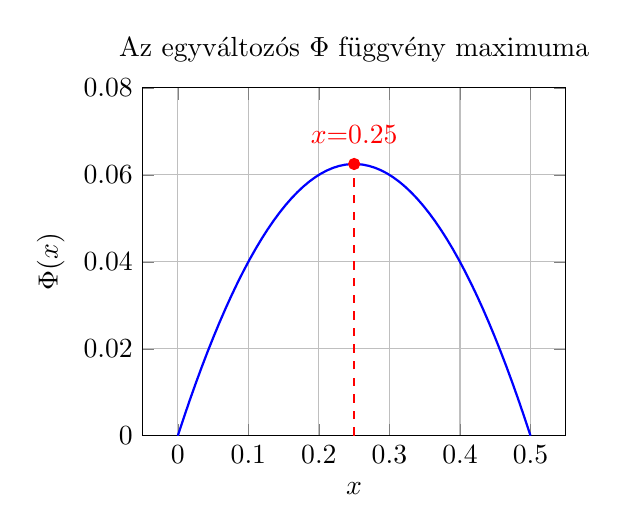
\begin{tikzpicture}
        \begin{axis}[
            title={Az egyváltozós $\Phi$ függvény maximuma},
            scaled ticks=false,
            tick label style={/pgf/number format/fixed},
            xlabel={$x$},
            ylabel={$\Phi(x)$},
            height=6cm,
            grid=major,
            ymin=0,
            ymax=0.08
        ]

        \addplot[blue, thick, domain=0:0.5, samples=60] {x*(0.5-x)};
        \addplot[red, dashed, thick] coordinates {(0.25,0) (0.25, 0.0625)};
        \addplot[only marks, mark=*, red] coordinates {(0.25, 0.0625)};
        \node[red, above] at (axis cs:0.25,0.065) {$x$=0.25};
            
        \end{axis}
    \end{tikzpicture}
\end{center}

\emph{Nagyon} informálisan nézve: itt azzal, hogy az $f$ függvény egyik változóját a másikból ki tudtuk fejezni (persze csak a leszűkítésen!), kvázi ``elcsaltunk'' egy dimenziót. A maradék dimenziónkban pedig tökéletesen tudunk mozogni minden irányba, kb. ``hozzáillesztve'' az ``elcsalt'' dimenzió-beli pozíciónkat. A fő különbség, hogy itt már nem tárol el az egyik függvény változó ``felesleges'' információt, azaz a belső pont megkötés élesedik arra az egy változónkra, ami az összes információt tartalmazza. Ez ellentétben áll az eredeti felállással, ahol azt vártuk volna el, hogy két, ``közös információt'' is tartalmazó, változó külön-külön is szabadon mozgatásával a halmazon belül maradjunk. A $h$ függvény bevezetésével ez megoldódik, mivel $\Phi$-ben a $h$ segítségével mi adjuk meg, hogy az egy változónk elmozgatása szerint a másikat hogyan kell módosítani (tulajdonképpen a ``közös információ'' alapján).

A fenti feladat ezzel az intuícióval több változóra is kiáltalánosítható, a feltételes szélsőérték (és később az implicitfüggvény) fogalmának bevezetésével.

\subsection{Definíció}

Legyen $1 \le n, m \in \N,\ \emptyset \ne U \subset \R^n$ és $f : U \to \R, g = (g_1,\,\ldots,\, g_m) : U \to \R^m$.

Ekkor $f$ függvénynek a \textbf{$g = 0$ feltételre vonatkozóan feltételes lokális maximuma (minimuma) van a $c \in \{g = 0\} := \{\xi \in U : g(\xi) = 0\}$ pontban}, ha az $\tilde f(\xi) := f(\xi)\quad (\xi \in \{g=0\})$ függvénynek $c$-ben lokális maximuma (minimuma) van.

Továbbá elnevezzük $f(c)$-t \textbf{feltételes lokális maximum (minimum)} vagy \textbf{szélsőérték}nek, és $c$-t pedig \textbf{feltételes lokális maximumhely (minimumhely)} vagy \textbf{szélsőértékhely}nek.

\subsubsection{Megjegyzések}

Feltesszük továbbá, hogy $\{g=0\} \ne \emptyset$,

A definícióban szereplő $\tilde f(\xi)$ az $f|_{\{g=0\}}$ leszűkítés.

\begin{samepage}
Tehát, ha $f$-nek egy $c \in \{g=0\}$ pontban lokális szélsőértéke van a $g=0$ feltételre nézve, akkor $\exists K(c)$, amire maximumnál $f(\xi) \le f(c)$, minimumnál $f(\xi) \ge f(c) \quad (\xi \in \{g=0\}\cap K(c))$.
\end{samepage}

\section{Feltételek}

\subsection{Elsőrendű szükséges feltétel}

\subsubsection{Tétel}

Legyen $1 \le n,m \in \N,\ m < n,\ \emptyset \ne U \subset \R^n$ nyílt és $f : U \to \R,\ g = (g_1,\,\ldots,\,g_m) : U \to \R^m$.

Továbbá tegyük fel, hogy

\begin{enumerate}[label=(\alph*),itemsep=1pt,topsep=1pt]
    \item $f \in D$
    \item $g \in C^1$
    \item $f$-nek $c\in\{g=0\}$ helyen feltételes lokális szélsőértéke van $g=0$ feltételre nézve
    \item $g'(c)$ Jacobi-mátrix rangja egyenlő $m$-mel
    ($\Leftrightarrow$ a gradiensvektorok lineárisan függetlenek),
    azaz $\rang g'(c) = m$. Ezt hívjuk \emph{rangfeltételnek}.
\end{enumerate}

Ekkor $\exists \lambda \in \R^m : \grad (f + \lambda g)(c) = 0$, ahol $\displaystyle(\lambda g)(\xi) := \dprod {\lambda,g(\xi)} = \sum_{i=1}^m \lambda_ig_i(\xi) \quad (\xi \in U)$.

Vegyük észre, hogy a tétel nagyon hasonló a feltétel nélküli esethez, csak itt a vizsgált $f$ függvény helyett az $f_\lambda := f + \lambda g$ függvényre vonatkozik. A $\lambda_i$-ket \textbf{Lagrange-multiplikátor} nevezzük, $f_\lambda$-t pedig \textbf{Lagrange-függvénynek}.  Hasonlóan fog felépülni a következő két tétel is.

\subsection{Másodrendű elégséges feltétel}

\subsubsection{Feltételes definitség}

A tétel kimondása előtt be kell vezetnünk a feltételes definitség fogalmát.

Legyen $Q : \R^n \to \R$ egy kvadratikus alak és $B \in \R^{m\times n}$. Vegyük az $\mathcal A_B := \{x \in \R^n : B\cdot x = 0\}$ halmazt.
Továbbá tfh. $m < n$ és $\rang B = m$.

Ekkor a $Q$ kvadratikus alak $B$-re nézve:
\begin{enumerate}[label=(\alph*),itemsep=1pt,topsep=1pt]
    \item \textbf{feltételesen pozitív definit}, ha $Q(x) > 0 \quad (0 \ne x \in \mathcal A_B)$
    \item \textbf{feltételesen negatív definit}, ha $Q(x) < 0 \quad (0 \ne x \in \mathcal A_B)$
    \item \textbf{feltételesen pozitív szemidefinit}, ha $Q(x) \ge 0 \quad (x \in \mathcal A_B)$
    \item \textbf{feltételesen negatív szemidefinit}, ha $Q(x) \le 0 \quad (x \in \mathcal A_B)$
\end{enumerate}

\subsubsection{Tétel}

\begin{samepage}

Legyen $1 \le n,m \in \N,\, m < n,\, \emptyset \ne U \subset \R^n$ nyílt és $f : U \to \R,\ g : U \to \R^n$. 
    
Továbbá tegyük fel, hogy
\begin{enumerate}[label=(\alph*), itemsep=1pt, topsep=1pt]
    \item $f,\,g \in D^2$
    \item $c \in \{g=0\}$-ben $\rang g'(c) = m$
    \item egy $\lambda \in \R^m$ vektorral vett $f_\lambda := f + \lambda g$-re:
    \begin{enumerate}[label=(\roman*),itemsep=1pt,topsep=1pt]
        \item $\grad f_\lambda(c) = 0$
        \item $Q_c^{f_\lambda}$ kvadratikus alak a $g'(c)$ mátrixra nézve feltételesen pozitív (negatív) definit
    \end{enumerate}
\end{enumerate}

Ekkor $f$-nek $c$-ben a $g=0$ feltételre vonatkozóan feltételes lokális minimuma (maximuma) van.

\end{samepage}

\subsection{Másodrendű szükséges feltétel}

\subsubsection{Tétel}

Legyen $1 \le n,m \in \N,\, m < n,\, \emptyset \ne U \subset \R^n$ nyílt, $f : U \to \R,\, g: U \to \R^m$ és $c \in \{g=0\}$.

Továbbá tegyük fel, hogy
\begin{enumerate}[label=(\alph*), itemsep=1pt, topsep=1pt]
    \item $f,\,g \in D^2$
    \item $\rang g'(c) = m$
    \item $f$-nek $c$-ben a $g=0$ feltételre vonatkozóan feltételes lokális minimuma (maximuma) van
\end{enumerate}

Ekkor $\exists \lambda \in \R^m$, amivel $f_\lambda := f + \lambda g$-re teljesül, hogy

\begin{enumerate}[label=(\alph*), itemsep=1pt, topsep=1pt]
    \item $\grad f_\lambda(c) = 0$
    \item $Q_c^{f_\lambda}$ kvadratikus alak $g'(c)$ mátrixra nézve feltételesen pozitív (negatív) szemidefinit
\end{enumerate}

\needspace{7\baselineskip}
\subsection{Megjegyzések}

\subsubsection{$m = n$ eset}

A feltételeknél $m < n$ feltevéssel éltünk, azonban könnyen belátható, hogy $m = n$ esetén is működnek az állítások. Nézzük például az elsőrendű szükséges feltételt.

\begin{samepage}
Ilyenkor $g'(c) \in \R^{n \times n}$ és a $\rang g'(c) = m = n$ rangfeltétel miatt a
$$
g'(c) = 
\begin{bmatrix}
\grad g_1(a) \\
\vdots \\
\grad g_n(a)
\end{bmatrix}
\in \R^{n \times n}
$$
Jacobi-mátrix \emph{invertálható.}
\end{samepage}

Vagyis a $\grad g_k(a) \in \R^n \ (k = 1,\ldots,n)$ vektorok lineárisan függetlenek, azaz bázist alkotnak $\R^n$-ben. Így bármilyen $\R^n$-beli vektor előállítható a lineáris kombinációjukként, spec.:
$$\exists! \lambda_j \in \R \enspace (j = 1,\ldots, n) : \sum_{j=1}^n \lambda_j \grad g_j(c) = -\grad f(c)$$

Tehát a $\lambda := (\lambda_1, \ldots, \lambda_n) \in \R^n$ vektorral teljesül, hogy $\grad (f + \lambda g)(c) = 0$. Ez alapján $n = m$ esetben is teljesül a tétel, azonban ott triviális.

\subsubsection{$\lambda$ és $c$ értékek meghatározása}

Szeretnénk felírni egy egyenletrendszert, amiből meghatározhatjuk a $\lambda_1,\ldots,\lambda_m$ és $c_1,\ldots,c_n$ értékeket. Ehhez $n + m$ darab egyenlet fog kelleni.

Vegyük az $\displaystyle f_\lambda := f + \lambda g = f + \sum_{k=1}^m \lambda_k \cdot g_k$ függvényt.

Az elsőrendű szükséges feltétel szerint $\grad f_\lambda(c) = 0$, amit ha kibontunk:

$$\partial_j f(c_1,\ldots,c_n) + \sum_{k=1}^m\lambda_k \partial_j g_k(c_1,\ldots,c_n)=0 \quad (j = 1,\ldots, n)$$

Ez összesen $n$ darab egyenletet fog adni. A maradék $m$ egyenletet a $g(c)=0$ feltételből kapjuk, ugyanis $g_l(c_1, \ldots,c_n) = 0 \quad (l = 1,\ldots,m)$.

\subsubsection{$\R^2$-beli feltételes definitség $g'(c)$-re nézve}\label{note:cond-orto}

Nézzük a $B := g'(c) \in \R^{m \times n}$, $m$-rangú mátrixszal vett $\mathcal A_B := \{y \in \R^n : B \cdot y = 0\}$ halmazt $m=1,\ n=2$ esetben:

Ekkor $0 \ne B = \grad g(c) \in \R^2$ és $\mathcal A_B = \{y \in \R^2 : \dprod{\grad g(c),\,y} = 0\}$.

Skaláris szorzat tulajdonságai alapján ekkor tudjuk, hogy $x \in \mathcal A_B$ azzal ekvivalens, hogy $x$ merőleges a gradiensre. Vagyis az $\mathcal A_B$ halmaz az origón átmenő, $\grad g(c)$ vektorra merőleges egyenes.

Hasonlóan $m=1,\, n > 2$ esetben pedig $\grad g(c)$ és $x$ ortogonálisak kell, hogy legyenek.

\subsubsection{Példafeladat}

Legyen $n := 2,\, m:=1,\,f(x,y) := 2x + 3y$ és $g(x,y) := x^2+y^2-1 \enspace \big((x,y) \in \R^2\big)$.

Ezek alapján definiáljuk $f_\lambda$-t: $f_\lambda(x,y) := 2x + 3y + \lambda(x^2+y^2-1) \enspace \big((x,y) \in \R^2\big)$.

Ekkor az elsőrendű szükséges feltétel szerint a következő egyenletrendszer megoldásaiban lehet csak feltételes lokális szélsőértéke a függvénynek $g = 0$ feltételre nézve:
\begin{alignat*}{2}
    \partial_1 f_\lambda(x,y) &= 2 + 2\lambda x &&= 0 \\
    \partial_2 f_\lambda(x,y) &= 3 + 2\lambda y &&= 0 \\
    g(x,y)                    &= x^2 + y^2 - 1  &&= 0
\end{alignat*}

Számoljuk ki az egyenletrendszer megoldásait:
\begin{gather*}
    x_1 := \frac 2 {\sqrt{13}},\ y_1 := \frac 3 {\sqrt{13}},\ \lambda_1 := -\frac {\sqrt{13}} 2,
    \\
    x_2 := -\frac 2 {\sqrt{13}},\ y_2 :=  -\frac 3 {\sqrt{13}},\ \lambda_2 := \frac {\sqrt{13}} 2
\end{gather*}

Ezekre teljesül, hogy $g'(x_i, y_i) = \grad g(x_i, y_i) = (2x_i, 2y_i) = 2(x_i, y_i) \quad (i = 1,2)$.

Valamint a $c^{(i)} := (x_i, y_i) \in \R^2 \enspace (i = 1,2)$ jelölés bevezetésével:
$$Q_{c^{(i)}}^{f_\lambda}(x,y) =
\dprod{
    \begin{bmatrix}
        2\lambda_i & 0 \\
        0 & 2\lambda_i
    \end{bmatrix}
    \cdot
    \xymat
,\, \xymat}
=
\dprod{
    \begin{bmatrix}
        2\lambda_ix \\
        2\lambda_iy
    \end{bmatrix},
    \xymat
}
=
2 \lambda_i(x^2 + y^2)$$

\begin{gather*}
Q_{c^{(1)}}^{f_\lambda}(x,y) = -\sqrt{13}(x^2+y^2) < 0
\enspace \text{és} \enspace
Q_{c^{(2)}}^{f_\lambda}(x,y) = \sqrt{13}(x^2+y^2) > 0
\\[4pt]
\big((x,y) \in \R^2 \setminus \{(0,0)\}\big)
\end{gather*}

Tehát $Q_{c^{(1)}}^{f_\lambda}$ negatív definit, $Q_{c^{(2)}}^{f_\lambda}$ pozitív definit, vagyis a másodrendű elégséges feltétel szerint $f$-nek $c^{(1)}$-ben feltételes lokális maximuma, $c^{(2)}$-ben feltételes lokális minimuma van.

\section{Elsőrendű szükséges feltétel bizonyítása}

\subsection{Tétel}

Legyen $1 \le n,m \in \N,\ m < n,\ \emptyset \ne U \subset \R^n$ nyílt és $f : U \to \R,\ g = (g_1,\,\ldots,\,g_m) : U \to \R^m$.

Továbbá tegyük fel, hogy
\begin{enumerate}[label=(\alph*),itemsep=1pt,topsep=1pt]
    \item $f \in D$
    \item $g \in C^1$
    \item $f$-nek $c\in\{g=0\}$ helyen feltételes lokális szélsőértéke van $g=0$ feltételre nézve
    \item $\rang g'(c) = m$
\end{enumerate}
Ekkor $\exists \lambda \in \R^m : \grad (f + \lambda g)(c) = 0$, ahol $\displaystyle(\lambda g)(\xi) := \dprod {\lambda,g(\xi)} = \sum_{i=1}^m \lambda_ig_i(\xi) \quad (\xi \in U)$.
\vspace{-18pt}
\subsection{Bizonyítás}

Egy gyors lebontása a ``szereplőinknek'', támpontnak a bizonyítás során:
\begin{itemize}[itemsep=1pt,topsep=1pt]
    \item $m < n$
    \item $U \subset \R^n$ nyílt
    \item $f : U \to \R$ (azaz $f \in \R^n \to \R$) és $f \in D$
    \item $g : U \to \R^m$ (azaz $g \in \R^n \to \R^m$) és $g \in C^1$
    \item $\{g=0\} \subset U \subset \R^n$
    \item $c \in \{g=0\}$, vagyis $c \in \R^n$
    \item $\rang g'(c) = m$
\end{itemize}

\subsubsection{Bizonyítás}

A rangfeltételből tudjuk, hogy $g'(c) \in \R^{m\times n}$ mátrixnak létezik $A \in \R^{m \times m}$ részmátrixa, amire $\det A \ne 0$ (mivel az összes ($m$ darab) sora lineárisan független). 

Jelöljük az $A$ mátrixot meghatározó oszlopok indexét $j_1, \ldots, j_m$-el, majd vegyük a következő indexhalmazt:
$$\{i_1, \ldots, i_{n-m}\} := \{1, \ldots, n\} \setminus \{j_1, \ldots, j_m\}$$
Ekkor $j_k \enspace (k = 1,\ldots,m)$ a lineárisan független oszlopokat indexeli, $i_k \enspace (k = 1,\ldots,n-m)$ pedig a maradékot.

Ha nehézséget okoz a bizonyítás megértése, vagy inkább az intuíció az egész mögött, akkor egy rövid, megértést remélhetőleg segítő szekció megtalálható a függelékben (ld. \ref{sec:cond-expl}), azonban ott használva vannak az eddig bevezetett jelölések.

\bigskip

Vezessük be eszerint az $\R^n \equiv \R^{n-m} \times \R^m$ felbontást, azaz
\begin{gather*}
    \xi = (\xi_1, \ldots, \xi_n) = (x,y) \in \R^n, \enspace \text{ahol} \\
    x := (\xi_{i_1},\ldots,\xi_{i_{n-m}}) \in \R^{n-m},\ y := (\xi_{j_1},\ldots,\xi_{j_m}) \in \R^m
\end{gather*}

Tehát tulajdonképpen itt az indexek által megadott permutáció szerint átrendeztük a mátrix oszlopait úgy, hogy $y$-ba kerüljenek a lineárisan független oszlopok, $x$-be pedig a maradék.\footnote{Belátható, hogy ez a permutáció nem lesz hatással semmilyen számunkra fontos tulajdonságra nézve. Ez az $i$ és $j$ szerinti indexelés a könyvből származik, a segédanyag egyszerűen felteszi, hogy $A$ az utolsó $m$ oszlopában áll elő $g'(c)$-nek, ekkor $x = (\xi_1,\ldots,\xi_{n-m}),\ y = (\xi_{n-m+1},\ldots,\xi_n)$. Vizsgán ennek is egy teljesen elfogadott módszernek kell lennie, persze indoklásnak kellhet, hogy meg tudunk adni egy $\sigma$ permutációt, ami ezt előállítja, majd a végén alkalmazni tudjuk $\sigma^{-1}$-t a tulajdonságok sérülése nélkül.}
% TODO: levezetés, hogy miért nem sérülnek a tulajdonságok?

Szedjük szét a felbontás szerint $c$-t is, $c = (a,b)$ komponensekre. Ekkor $\partial_2 g(a,b) = A$, amiről tudjuk, hogy invertálható, vagyis $\det \partial_2 g(a,b) \ne 0$ következik. Továbbá $c \in \{g=0\}$ miatt $g(a,b) = 0$, így alkalmazhatjuk az implicitfüggvény-tételt.

Ekkor alkalmas $K(a) \subset \R^{n-m},\ K(b) \subset \R^m$ környezetekkel létezik $g$ által az $(a,b)$ körül meghatározott $h : K(a) \to K(b)$ implicitfüggvény, amire $h \in C^1$ és
$$h'(x) = -\Big(\partial_2g(x,h(x))\Big)^{-1} \cdot \partial_1g(x,h(x)) \quad (x \in K(a))$$

Világos\footnote{
Annyira nem, tekintve hogy ez az állítás egyáltalán nem tartja tiszteletben a fenti permutációnkat, de nem aggódunk túlságosan emiatt, mivel a könyv se aggódott túlságosan emiatt.
}, hogy ha a $\{g=0\}$ halmazt leszűkítjük ezekre a környezetekre, akkor
$$\big(K(a) \times K(b)\big)\cap \{g=0\} = \{(x,\,h(x)) \in U : x \in K(a)\}$$

Mivel $c$ feltételes lokális szélsőértéke $f$-nek $g=0$-ra nézve, így $f(\xi) \le f(c) \enspace (\xi \in K(c) \cap \{g=0\})$.\footnote{
Itt most feltettük, hogy $f(c)$ feltételes lokális maximum. Minimumra természetesen ezzel analóg módon történik a levezetés.
}

Feltehető $K(a) \times K(b) \subset K(c)$.

Definiáljuk a $\Phi(x) := f(x,\, h(x)) \enspace (x \in K(a))$ függvényt, amire $\Phi(x) \le f(c) = \Phi(a)$ teljesül, bármely $x \in K(a)$ mellett. Tehát $\Phi$-nek lokális maximuma van $a$-ban. 

Mivel $\Phi \in D(K(a))$ is teljesül, így
$$\Phi'(a) = \grad \Phi(a) = 0$$

Vezessük be a $\varphi(x) := (x, h(x)) \enspace (x \in K(a))$ függvényt, amivel $\Phi = f \circ \varphi$. Teljesül továbbá $\varphi \in D$, valamint ha $I$ az $\R^{(n-m)\times(n-m)}$ egységmátrixot jelöli, akkor
$$\varphi'(x) = \begin{bmatrix}I \\ h'(x)\end{bmatrix} \in \R^{n\times(n-m)}\qquad (x \in K(a))$$

A fentiek, és az összetett függvények deriváltja tétel alapján,

\begin{gather*}
    0 = \Phi'(a) = f'(\varphi(a)) \cdot \varphi'(a) = f'(a,h(a)) \cdot \begin{bmatrix}I \\ h'(a)\end{bmatrix} = f'(c) \cdot \begin{bmatrix}I \\ h'(a)\end{bmatrix} = \\
    \partial_1f(c) + \partial_2f(c)\cdot h'(a) = \partial_1f(c) - \partial_2f(c) \cdot \big(\partial_2g(c)\big)^{-1}
\cdot \partial_1g(c)\end{gather*}

Ekkor legyen $\lambda := -\partial_2f(c)\cdot\big(\partial_2g(c)\big)^{-1} \in \R^m$, ezzel $0 = \partial_1 f(c) + \lambda\cdot\partial_1g(c)$.

Továbbá $\big(\partial_2g(c)\big)^{-1}$-el ``átszorozva'' kapjuk, hogy: $\partial_2f(c) + \lambda \cdot \partial_2g(c) = 0$.

Ebből a $\partial_1$ és $\partial_2$ tagokat kibontva kapjuk a következő egyenlőségeket:
\begin{align*}
\partial_{i_k}f(c) + \sum_{l=1}^m \lambda_l\cdot\partial_{i_k}g_l(c) &= 0 \quad (k=1,\ldots,n-m) \\
\partial_{j_k}f(c) + \sum_{l=1}^m \lambda_l \cdot \partial_{j_k}g_l(c) &= 0 \quad (k=1,\ldots,m)
\end{align*}

Ezeket összevonva pedig:
$$\partial_k f(c) + \sum_{l=1}^m \lambda_l \cdot \partial_kg_l(c) = 0 \quad (k = 1,\ldots,n)$$

Tehát $\displaystyle \grad (f + \lambda g)(c) = \left( \partial_1f(c) + \sum_{l=1}^m \lambda_l \cdot \partial_1g_l(c), \ldots, \partial_n f(c) + \sum_{l=1}^m \lambda_l \cdot \partial_n g_l(c) \right) = 0$. \qed